\ProvidesPackage{preamble}
\usepackage[utf8]{inputenc}
\usepackage[T1]{fontenc,url}
\usepackage{babel,textcomp}
\usepackage{graphicx}
\usepackage{pdfpages}
\usepackage{fancyhdr}
\usepackage{afterpage}
\usepackage{amsmath}
\usepackage{amssymb}
\usepackage{caption}
\usepackage{mathtools}
\usepackage{listings}
\usepackage{color}
\usepackage[margin=1.2in]{geometry}

%\usepackage[hidelinks]{hyperref} % make links black
\usepackage{hyperref}
%\hypersetup{
  %colorlinks=false,
  %colorlinks=true,
  % citecolor=black,
  % filecolor=black,
  % linkcolor=red,
  % urlcolor=blue,
  % linktoc=all,
  % linktocpage,
%}

\pagestyle{fancy}
\fancyhead{}
\fancyfoot{}
\renewcommand{\headrulewidth}{0.0pt}
\renewcommand{\footrulewidth}{0.0pt}
\fancyhead[R]{\thepage}
\fancyhead[L]{\emph{}}

\renewcommand{\vec}[1]{\mathbf{#1}}    % vektorer i bf fremfor pil
\let\oldhat\hat
\renewcommand{\hat}[1]{\oldhat{\mathbf{#1}}} % enhetsvektorer i bf med hatt

\definecolor{keywords}{RGB}{50,50,250}
\definecolor{comments}{RGB}{190,70,20} % Orange
\definecolor{red}{RGB}{160,0,0}
\definecolor{green}{RGB}{0,150,0}
\definecolor{grey}{RGB}{225,225,225}

\lstdefinestyle{terminal}
{
  frame=single,
  basicstyle=\ttfamily,%\small,
}

\lstdefinestyle{fortran}
{
  frame=shadowbox,
  rulesepcolor=\color{black},
  language=Fortran,
  basicstyle=\ttfamily,%\small,
  keywordstyle=\bf\color{keywords},
  morekeywords={as,range,len,float},
  commentstyle=\color{comments},
  stringstyle=\color{red},
  showstringspaces={false}
}

\lstdefinestyle{python}
{
  %frame=shadowbox,
  rulesepcolor=\color{black},
  language=Python,
  basicstyle=\ttfamily,%\small,
  keywordstyle=\bf\color{keywords},
  morekeywords={as,range,len,float},
  commentstyle=\color{comments},
  stringstyle=\color{red},
  showstringspaces={false}
}
  % numbers=left,                     # Numbered lines
  % numbersep=5pt,                    # Dist from num to code
  % numberstyle=\small,%\color{mygray},
  % identifierstyle=\color{green}%,
  % backgroundcolor=\color{},
  % emph={MyClass,__init__},          % Custom highlighting
  % emphstyle=\ttb\color{deepred}}    % Custom highlighting style

% Custom commands
\newcommand{\pder}[2]{\frac{\partial #1}{\partial #2}}
\newcommand{\ppder}[2]{\frac{\partial^2 #1}{\partial^2 #2^2}}
\newcommand{\half}{\frac{1}{2}}
\newcommand{\intO}{\int_{\Omega}}
\newcommand{\intdO}{\int_{\partial\Omega}}
\newcommand{\intu}{\int^1_{-1}}
\newcommand{\ti}[1]{\tilde{#1}}
\newcommand{\md}{\;\mathrm{d}}
\newcommand{\ha}[1]{\text{\^{#1}}}

\title{
	{Thesis Title}\\
	{\large Institution Name}\\
}
\author{Author Name}
\date{Day Month Year}

\usepackage{amsmath,amsfonts,amssymb,amsthm,epsfig,epstopdf,titling,url,array}
\theoremstyle{definition}
\newtheorem{defn}{Definition}[section]
\newtheorem{conj}{Conjecture}[section]
\newtheorem{exmp}{Example}[section]
\usepackage{amsmath}                                    
\title{Benchmark}
\author{Sebastian Gjertsen}
\begin{document}
\maketitle
\section*{Problem Defintion}
\subsection*{Domain}
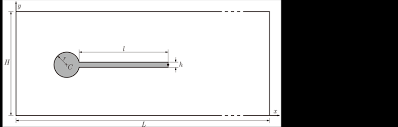
\includegraphics[scale=0.9]{geometry.png}
The computational domain resembles the classic cfd benchmark with an added bar, with dimensions:
The box: L = 2.5, H = 0.41
The bar: l = 0.35, h = 0.02
The circle is positioned at (0.2, 0.2) making it 0.05 of center from bottom to top, this is done to induce oscillations to a otherwise laminar flow.

\section*{Fluid Structure Interaction Problem formulation in ALE coordinates}
\includegraphics[scale=0.4]{continuum_mapping.png}

To get a monolithic ALE formulation, we need to define a mapping, in the solid domain:
$$  \chi^s(t) : \hat{\mathcal{S}} \rightarrow \mathcal{S}(t)     $$ 
We define the $ \hat{\mathcal{S}}$ as the initial stress free configuration, the $\mathcal{S}$ as the reference and the $\mathcal{S}(t)$ as the current configuration.
The same is for the fluid domain.
$$  \chi^f(t) : \hat{\mathcal{F}} \rightarrow \mathcal{F}(t)     $$ 
The solid mapping is set as $\chi^s(\textbf{X},t) = \textbf{X}  + d^s(\textbf{X} ,t)$
hence giving:
$$  d^s(\textbf{X},t) = \chi^s(\textbf{X},t) -\textbf{X}   $$
$$  w(\textbf{X},t) = \frac{\partial \chi^s(\textbf{X},t)}{\partial t}   $$

where $\textbf{X}$ denote a material point in the reference domain and $\chi^s$ denotes the mapping from the reference configuration.
We denote $\Gamma^1$ as the "ceiling" and "floor" and the circle and $\Gamma^{2,3}$ as the inlet and outlet.
The velocity in the fluid is denoted $u(\textbf{X},t)$
We define the deformation gradient $F = I + \nabla d$ and $J = det(F)$
\subsection*{Balance laws}
We will formulate the equations in the Eulerian, Lagrangian and the ALE description.
The Eulerian description suits a fluid problem nicely as the points in the grid are fixed and the fluid particles move through the domain. Whilst the Lagrangian description fits a solid problem as the material particles are fixed with the gridpoints. The fluid velocity vector and the displacement vector are the quantities describing motion of the fluid and solid respectively. Since we here have fluid structure interaction problem we need to formulate the fluid in the ALE description. The fluid velocity will still be the quantity describing motion but it will also have the displacement of the fluid, describing the change in fluid domain. The solid will be described in Lagrangian. We will only look at incompressible fluids where the volume of the fluid domain never change.\\
We express the solid balance laws in the Lagrangian formulation from the initial configuration
$$J\rho_s \frac{\partial^2 d}{\partial t^2} = \nabla \sigma_s(d) \hspace{4mm}in\hspace{4mm} \mathcal{\hat{S}} $$
The fluid equations are denoted from the initial configuration:
$$ \rho_s J \big( \frac{\partial u}{\partial t} + (\nabla u)F^{-1}(u-w)\big) = \nabla \cdot (J\sigma_f F^{-T} )\hspace{4mm} in \mathcal{\hat{F}}$$
$$ \nabla \cdot (J u F^{-T}) = 0 \hspace{4mm} in \hspace{2mm} \mathcal{\hat{F}}$$

To bind together the computation of fluid and structure domain, we need a harmonic extension to the boundary values. For this purpose define the following equation with the fluid domain deformation:
$$ \nabla^2 d^f = 0\hspace{4mm}in \hspace{2mm} \mathcal{\hat{F}}$$
This equation is chosen for its good regularity and smoothing properties.

Boundary conditions:
The fluid velocity has a given value on the inlet:
$$ u = u0 \hspace{4mm}on \hspace{2mm} \Gamma^2$$
We set no slip on the "floor" and "ceiling" so to speak:
$$ u = 0  \hspace{4mm}on \hspace{2mm} \Gamma^1  $$
In the place where the fluid and structure domains meet, i.e the interface. We set a dynamic condition saying that the normal stresses of the solid and fluid are equal:
$$  \sigma_f n_s = \sigma_s n_f \hspace{4mm} on  \hspace{2mm}\Gamma^0 (interface)   $$
\subsection*{Variational formulation}
We use 4 testfunctions, $\phi, \psi, \epsilon, \gamma$.
\begin{align*}
\rho_s J \big( \frac{\partial u}{\partial t} + (\nabla u)F^{-1}(u-w) , \phi\big)_{\mathcal{\hat{F}}} + (J\sigma_f F^{-T},\nabla \phi )_{\mathcal{\hat{F}}} &= 0  \\
 \big( \nabla \cdot (J u F^{-T}),\gamma \big)_{\mathcal{\hat{F}}} &= 0 \\
\big(J\rho_s \frac{\partial^2 d}{\partial t^2},\psi \big)_{\mathcal{\hat{S}}} + \big(F \sigma_s(d), \nabla \psi \big)_{\mathcal{\hat{S}}} &=0 \\
 \big( \nabla d , \nabla \epsilon \big)_{\mathcal{\hat{F}}} &= 0 \\
 \big( w- \frac{\partial d}{\partial t} ,\epsilon \big)_{\mathcal{\hat{S}}} &= 0 \\
 \text{Or we can change the last two with:  ??????} & \\ 
 \big( \nabla (dt\cdot w + d^0) , \nabla \epsilon \big)_{\mathcal{\hat{F}}} &= 0 
\end{align*}


\end{document}
